% Define the document type and special pacages
%--------------------------------------------------------%
\documentclass[12pt]{article}
\usepackage[utf8]{inputenc}

\title{Reseach Course on Detector technology - Semiconductor detector}
\author{Daniel S. Nielsen, Rosanna Ignazzi, \\Étienne Bourbeau, Fabian A.J. Thiele}
\date{\today}

\usepackage{listings}
\usepackage{color}
\usepackage[pdftex]{graphicx}
\usepackage{siunitx} % SI units
\usepackage{amsmath} % equations
\usepackage{tabularx}
\usepackage{tikz}
\usepackage{hyperref}
\usepackage{ifthen}
\usepackage[T1]{fontenc} % proper underscores etc.
\usepackage{subcaption} % replace subfloat with subfigure env.
\sisetup{per-mode=fraction}
\setlength{\parskip}{.8em} 
\usepackage{float}  %allows use of 'H' in the figure location

\begin{document}
% === Front matter ====================================================

%\frontmatter
\maketitle

\clearpage
  
\tableofcontents
  
%\listoffigures
  
%\listoftables
  
%\lstlistoflistings
  
\cleardoublepage

%################################################################################################
%
% Introduction
%
%################################################################################################

\section{Introduction}

Semiconductor detectors made of silicon are often used in particle physics. Their compact form and fast response to electronic signal makes them well suited for tracking detectors, such as the SCT detector of the ATLAS experiment at CERN.

When charged particles or ionizing radiation travels through a cell of such tracking detector, an ionizing current is created out of pairs of \textit{electrons} and \textit{holes}, which are collected at opposite electrodes with the help of a voltage potential applied to the device. Based on the timing and amplitude of the resulting signal, it is possible to estimate the energy deposited in the cell, as well as the initial direction of the ionizing particle.

Because of the small intensity of the original current produced in a semiconductor detector, preamplifiers and other readout electronics need to be used in conjunction with the tracking cells. This implies that proper calibration measurements must be made for the entire experimental assembly, in order for the data analysis to yield trustworthy and accurate results.

This report presents the details of the production and characteriztion of a PN-junction / preamplifier circuit. The production of a silicon diode is briefly described, along with its integration onto a pre-amplifier circuit board. A characterization of the noise and parasitic capacitance of both elements (sensor + preamplifier) is presented, along with the results of measurements taken with a radioactive source, on the fully assembled detector. 

%################################################################################################
%
% Methods
%
%################################################################################################

\section{Sensor preparation and characterization}

We worked on a p-type silicon detector. The silicon chip was provided without any connections between the top and bottom electrodes. To make these connections, the chip was sent to a clean room where wires were ultrasonically bonded to the top of the chip and the side electrode contacts. Once the wire bonding was done, the sensor was placed inside a probing station and kept in a dark environment for a series of characterization measurements.

Before integrating the silicon detector inside the rest of the circuit, several properties of the junction had to be measured, namely the \textit{depletion voltage} (the voltage at which the sensor is subjected to a reverse bias that is high enough to drain out all intrinsic carriers from the semiconductor), the \textit{leakage current} (undesired currents that add background to the signal current), and the \textit{capacitance} at depletion. All curves were measured $4$ times, in order to have an estimate of the uncertainty of each measurement.

To determine the depletion voltage, a bias scan was performed, and the current was measured with a pico amp-meter, as shown in the bottom plot of figure \ref{fig:IVcurve}. The depletion voltage was then defined to be -60V, and corresponds to the onset of the plateau region of the IV curve, which occurs when the width of the space charge region covers the entire width of the semiconductor.

\begin{figure}[H]
  \centering
  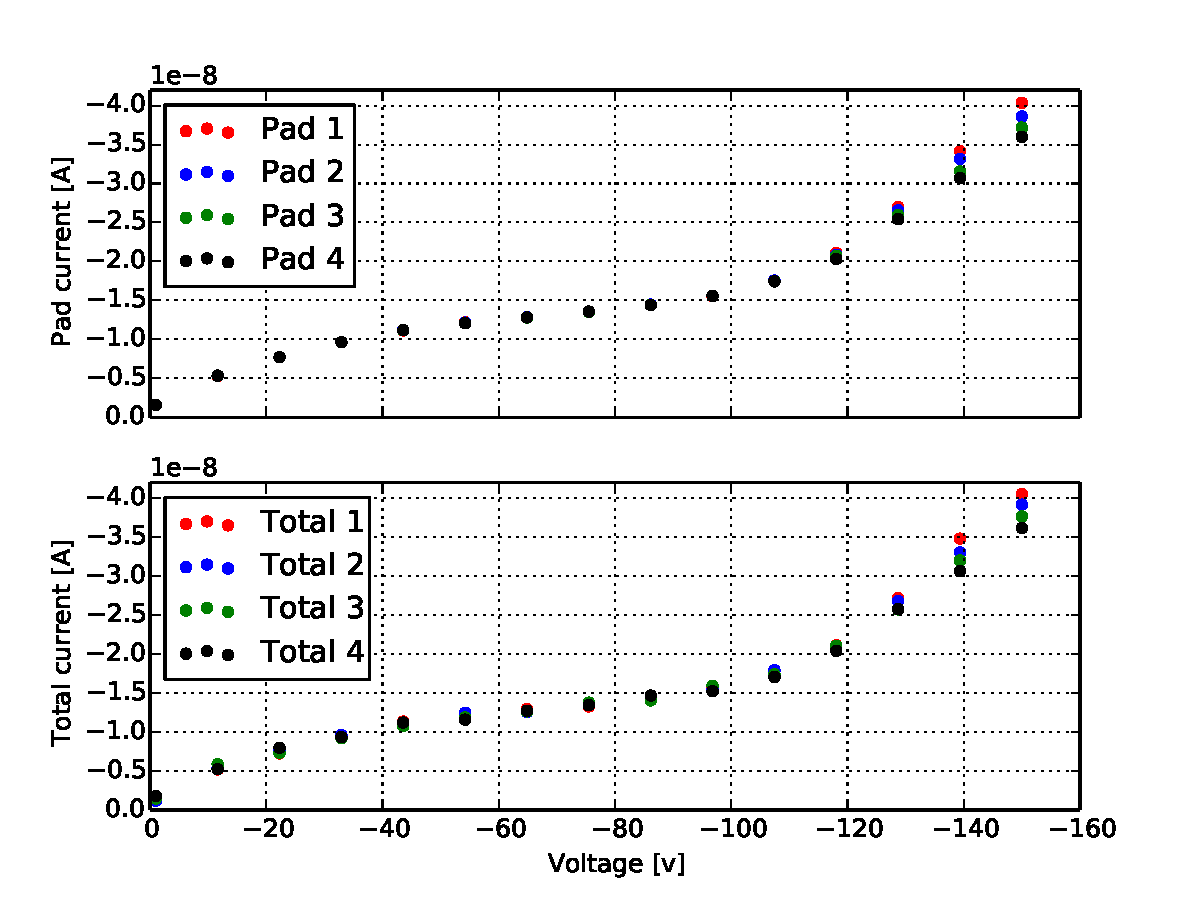
\includegraphics[width=0.8\textwidth]{./graphics/IV_V_vs_A.pdf}
  \caption{IV curve for the silicon detector of p-type. The upper plot shows the current per pad for the $4$ different pads, while the lower plot shows the total current }
  \label{fig:IVcurve}
\end{figure}

The same probing station was also used to measure the capacitance of the sensor. First, the parasitic capacitance of the measurement electronics was measured by monitoring the capacitance between the two contacts (in this case needles) of the probing station. The result of this scan is shown as the ``Open Needle'' line of figure \ref{fig:VC_curve_single}. Then, the capacitance of the sensor was measured as a function of voltage and the parasitic capacitance was subtracted, to get the correct value of the capacitance of the silicon detector. All measurements were performed four times, in order to gain insight on the uncertainty of the measurements. The capacitance of the diode at full depletion voltage ( $\approx 60$ V) is measured to $11.20 \pm 0.02$ pF, see Figure \ref{fig:VC_curve_single}.


\begin{figure}[H]
  \centering
  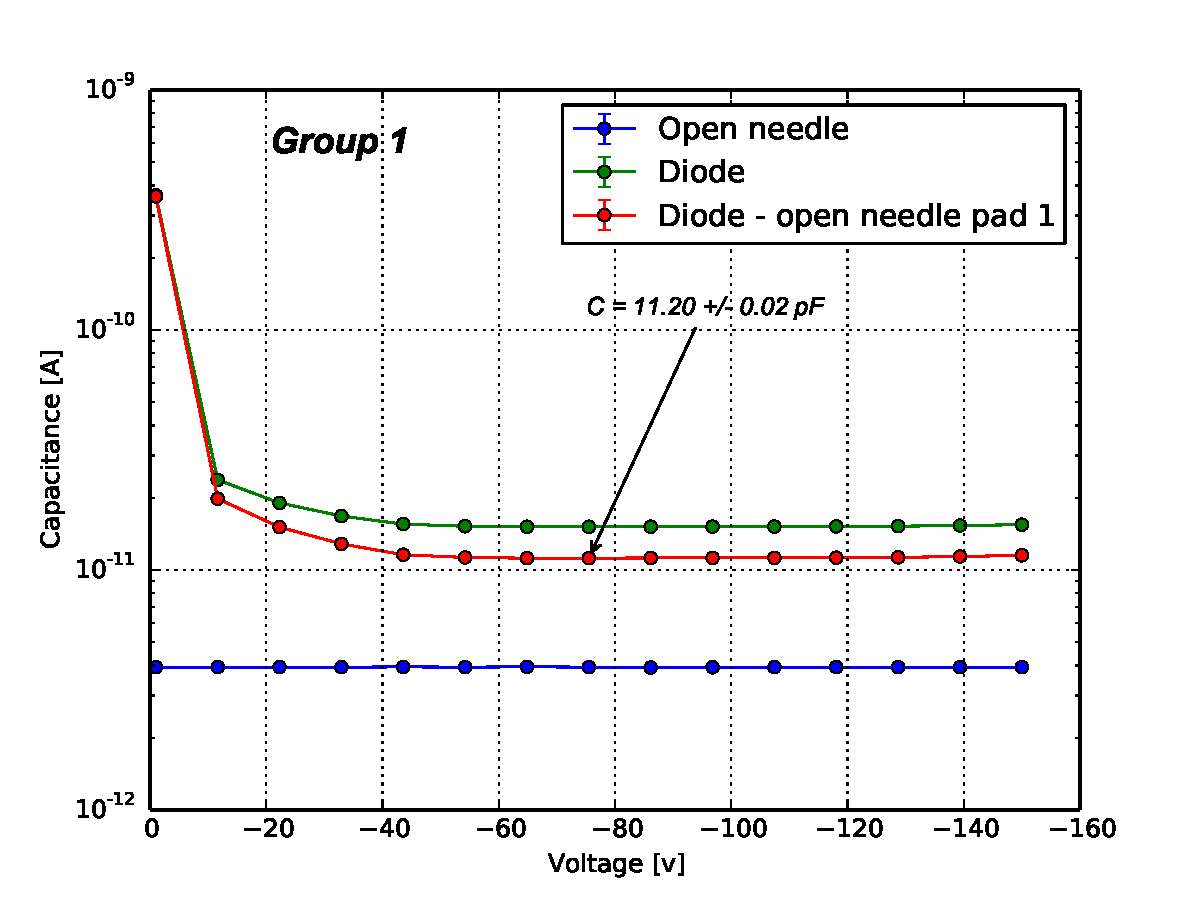
\includegraphics[width=0.8\textwidth]{./graphics/V_vs_C}
  \caption{Parasitic capacitance of the instrument (blue), capacitance of the system plus the silicon diode and capacitance of the diode as a function of voltage.}
  \label{fig:VC_curve_single}
\end{figure}



\section{Preamplifier Calibration}

Before attaching the sensor to the rest of the circuit to perform measurements, the response of the pre-amplifier was calibrated using the set-up illustrated in figure \ref{fig:preampsetup}. Different load capacitances between $1$ pF and $100$ pF were put in parallel to the capacitance of $0.4$ pF of the calibration input. The amplifier was supplied with two voltage biases of + and -12V from a DC workbench power supply. For every capacitance value, two quantities were measured: the RMS of the baseline noise when no pulse are injected, and the properties of the amplaified signal when provided with a calibrated pulse.  The circuit was fed with a square pulse of amplitude $20$ mV and the rise time of the output signal was measured directly on the oscilloscope between the $10\%$ and $90\%$ of the rising signal. The amplitude of the signal was noted as well. During these measurements, the circuit and the cables were coated with aluminium foil (grounded through a cable to the HV power supply), in order to shield the system from electrical interference that would cause additional noise to the output signal.

\begin{figure}[H]
  \centering
  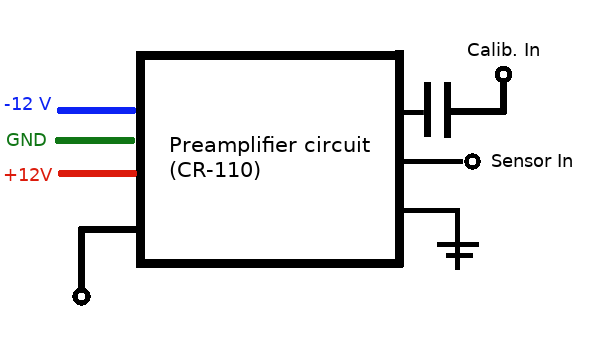
\includegraphics[width=0.8\textwidth]{./graphics/experimental_preamp_setup.png}
  \caption{Experimental setup of the preamplifier circuit}
  \label{fig:preampsetup}
\end{figure}


The noise-only measurements were recorded and plotted on Figure \ref{fig:Noise_vs_Capacitance}. As it is clearly visible, the noise RMS increases as a function of the input load capacitance.

\begin{figure}[H]
 \centering
  \begin{subfigure}[b]{\textwidth}
    \centering
    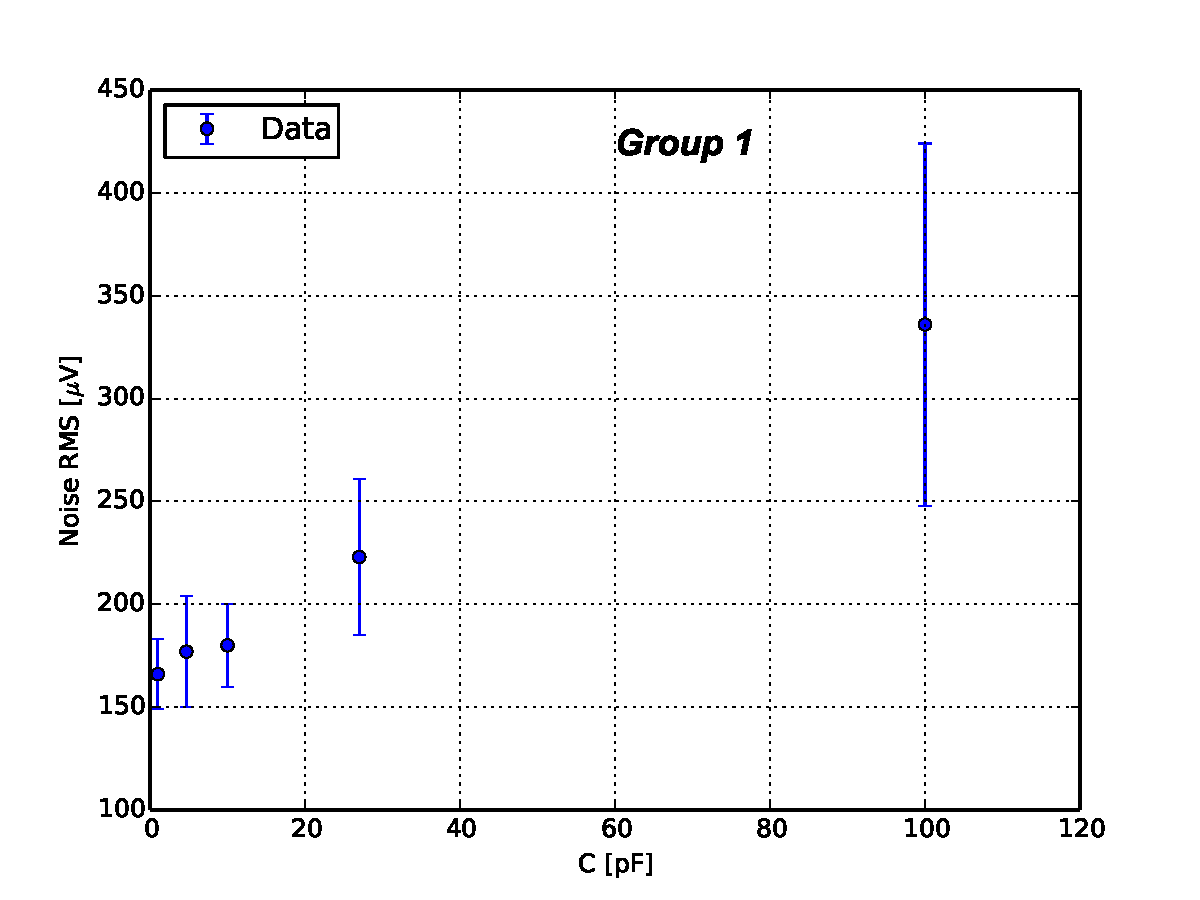
\includegraphics[width=0.8\textwidth]{./graphics/noise_vs_capacitance}
    \caption{Noise RMS vs capacitance}
    \label{fig:Noise_vs_Capacitance}
  \end{subfigure}
  
  \begin{subfigure}[b]{\textwidth}
    \centering
    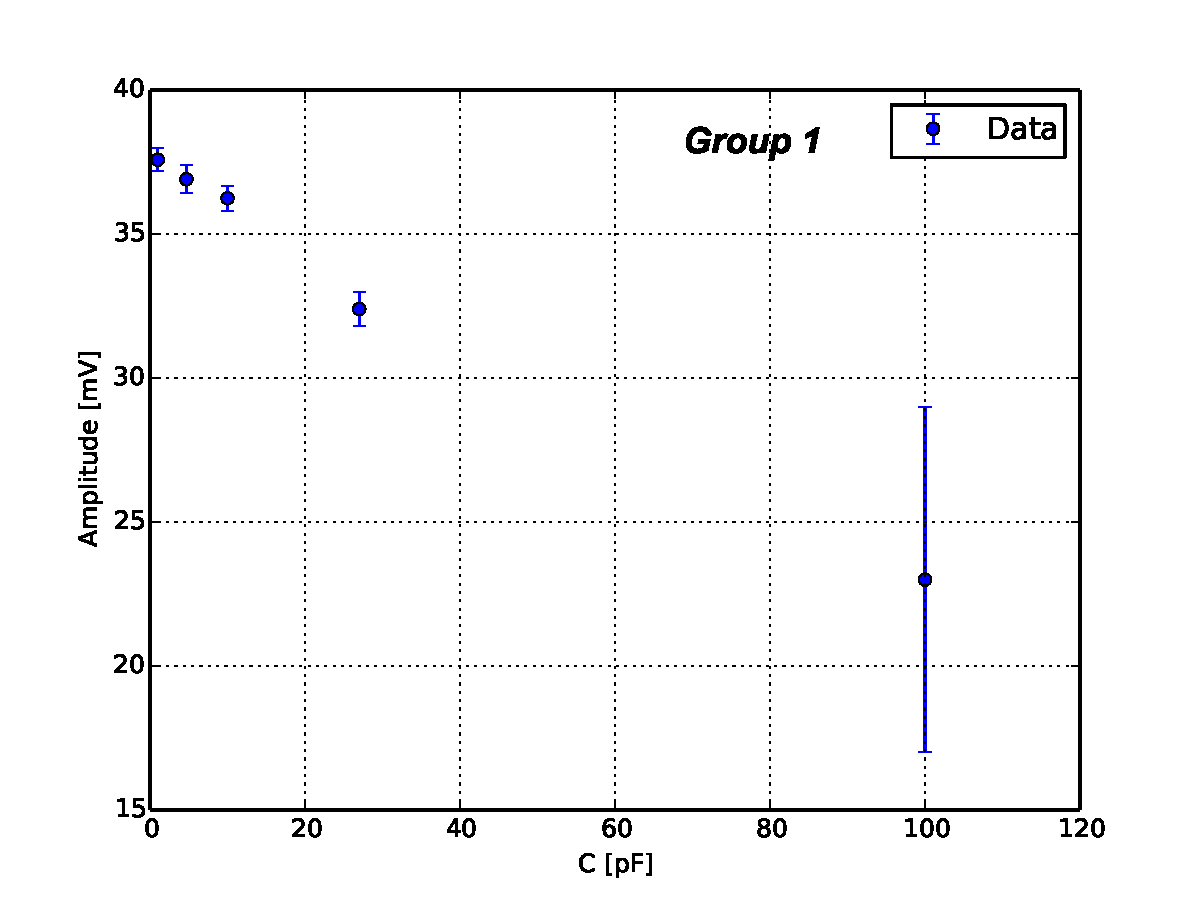
\includegraphics[width=0.8\textwidth]{./graphics/amplitude_vs_capacitance}
    \caption{Amplitude vs capacitance}
    \label{fig:Amplitude_vs_Capacitance}
  \end{subfigure}
  \caption{Calibration measurements for the pre-amplifier.}
  \label{fig:calib_others}
\end{figure}

  The amplitude and rise time of the output pulses are plotted as a function of circuit capacitance in figure \ref{fig:Amplitude_vs_Capacitance} and figure \ref{fig:RiseTime_vs_Capacitance} respectively. The rise time was measured by finding the time interval between the $10\%$ and $90\%$ of the rising pulse. As can be seen, the amplitude decreases as a function of load capacitance, while the rise time increases, which means that the pulse reacts more slowly  and loses some of its power as the circuit capacitance increases.

 One can note that at higher capacitance the measurements get more affected more by the noise, as it is visible by the errorbar size for C = $100$ pF for example. The rise time measurement was fitted to a $2$nd degree polynomial and the resulting paramters are shown in Figure \ref{fig:RiseTime_vs_Capacitance}

\begin{figure}[H]
  \centering
  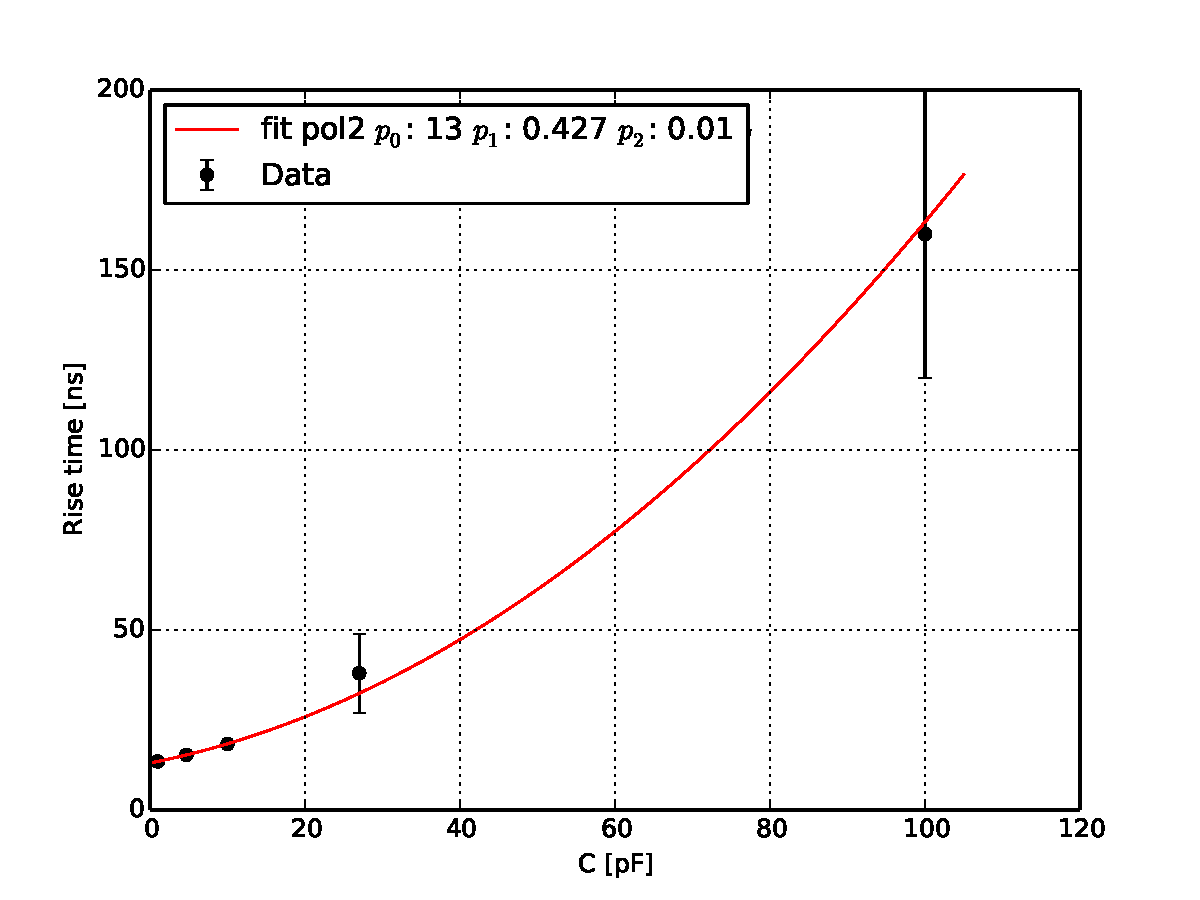
\includegraphics[width=0.8\textwidth]{./graphics/calibration_diode}
  \caption{Calibration of the rise time as a function of capacitance} %%% Add chi2 and errors on the pol2 parameters
  \label{fig:RiseTime_vs_Capacitance}
\end{figure}



\subsection{Equivalent Noise Charge}

The \textit{Equivalent Noise Charge}, or ENC, is the amount of charge one would have to inject into the pre-amplifier in order to match the recorded noise level of the output. In other words, we want to figure out, for a given capacitance, what the RMS noise signal would look like if it were an unamplified input signal. The ENC can be calculated as:
\begin{equation}
ENC = \frac{V_{rms}\cdot C_{calibration}}{G}
\end{equation}
where $V_{rms}$ is the voltage noise RMS, $C_{calibration}$ are the different capacitances used in the calibration procedure and $G$ is the gain.
The gain is given by the ratio of output-to-input voltage:
\begin{equation}
ENC = \frac{V_{in}}{V_{out}}\cdot\left(C_{calibration}\cdot V_{rms}\right)
\end{equation}
where $V_{in}$ is the input voltage of the calibration pulse and $V_{out}$ is the registered output voltage.
During the calibration test, the input voltage is fixed to $20$ mV, so the only thing that varies in this expression should be the capacitance. In practice though, the noise level and the output amplitude depend on the capacitance as well, as shown in Figure \ref{fig:Noise_vs_Capacitance} and \ref{fig:Amplitude_vs_Capacitance}.

\begin{figure}[H]
  \centering
  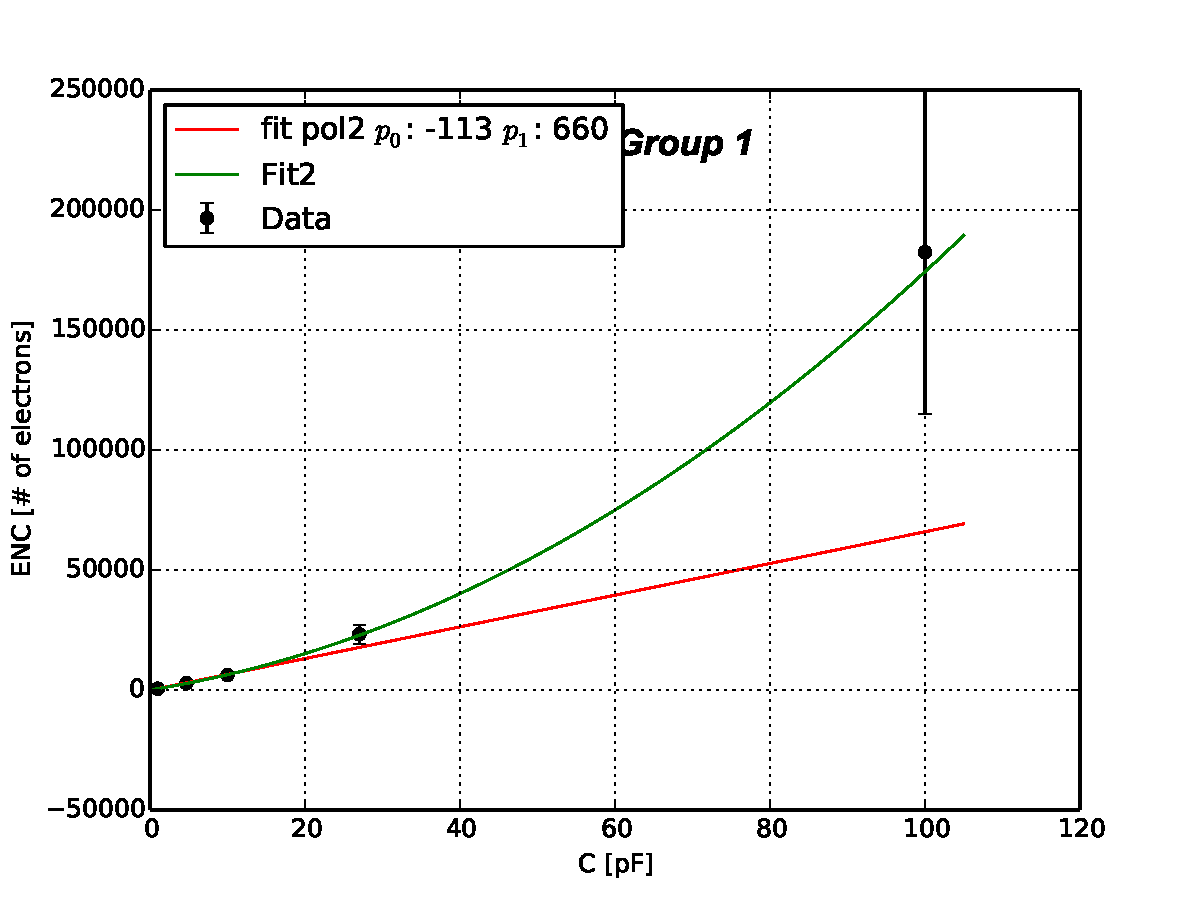
\includegraphics[width=0.8\textwidth]{./graphics/calibrationENC_diode}
  \caption{Calibration of the ENC as a function of capacitance} %%% Add chi2 and errors on the pol2 parameters
  \label{fig:ENC_vs_Capacitance}
\end{figure}

The ENC for the setup with the different capacitors was evaluated and the results can be seen in figure \ref{fig:ENC_vs_Capacitance}. It is clear that the ENC increases as a function of capacitance and this increase seems linear in the first points, while the last data point, due to the relatively high uncertainty, makes the linear fit less appropriate. The ENC at $0$ pF, given by the intercept in the linear fit, is $-113$ electrons.


\section{Final Assembly}
After the calibration measurements were completed, the silicon detector was introduced in the circuit by connecting it to the pre-amplifier. A voltage of around $60$ V was fed to the sensor, in order to fully deplete it, and the output was connected to a low-pass filter consisting of a $100$ nF capacitance and of a $300$ k$\Omega$ resistor, see Figure \ref{fig:ExperimentalSetup}. The resulting circuit is schematically shown in Figure \ref{fig:SiliconDiodeCircuit}.
Finally the Strontium-90 source was attached with tape to the lid of the box containig the entire circuit. By closing the lid and covering it with aliminium foil, external radiations were shielded. The measurement of the pulses induced in the silicon detector by the particles radiated by the Strontium decay were registered from the oscilloscoper for further analysis.

\begin{figure}[H]
  \centering
  \begin{subfigure}[b]{0.5\textwidth}
    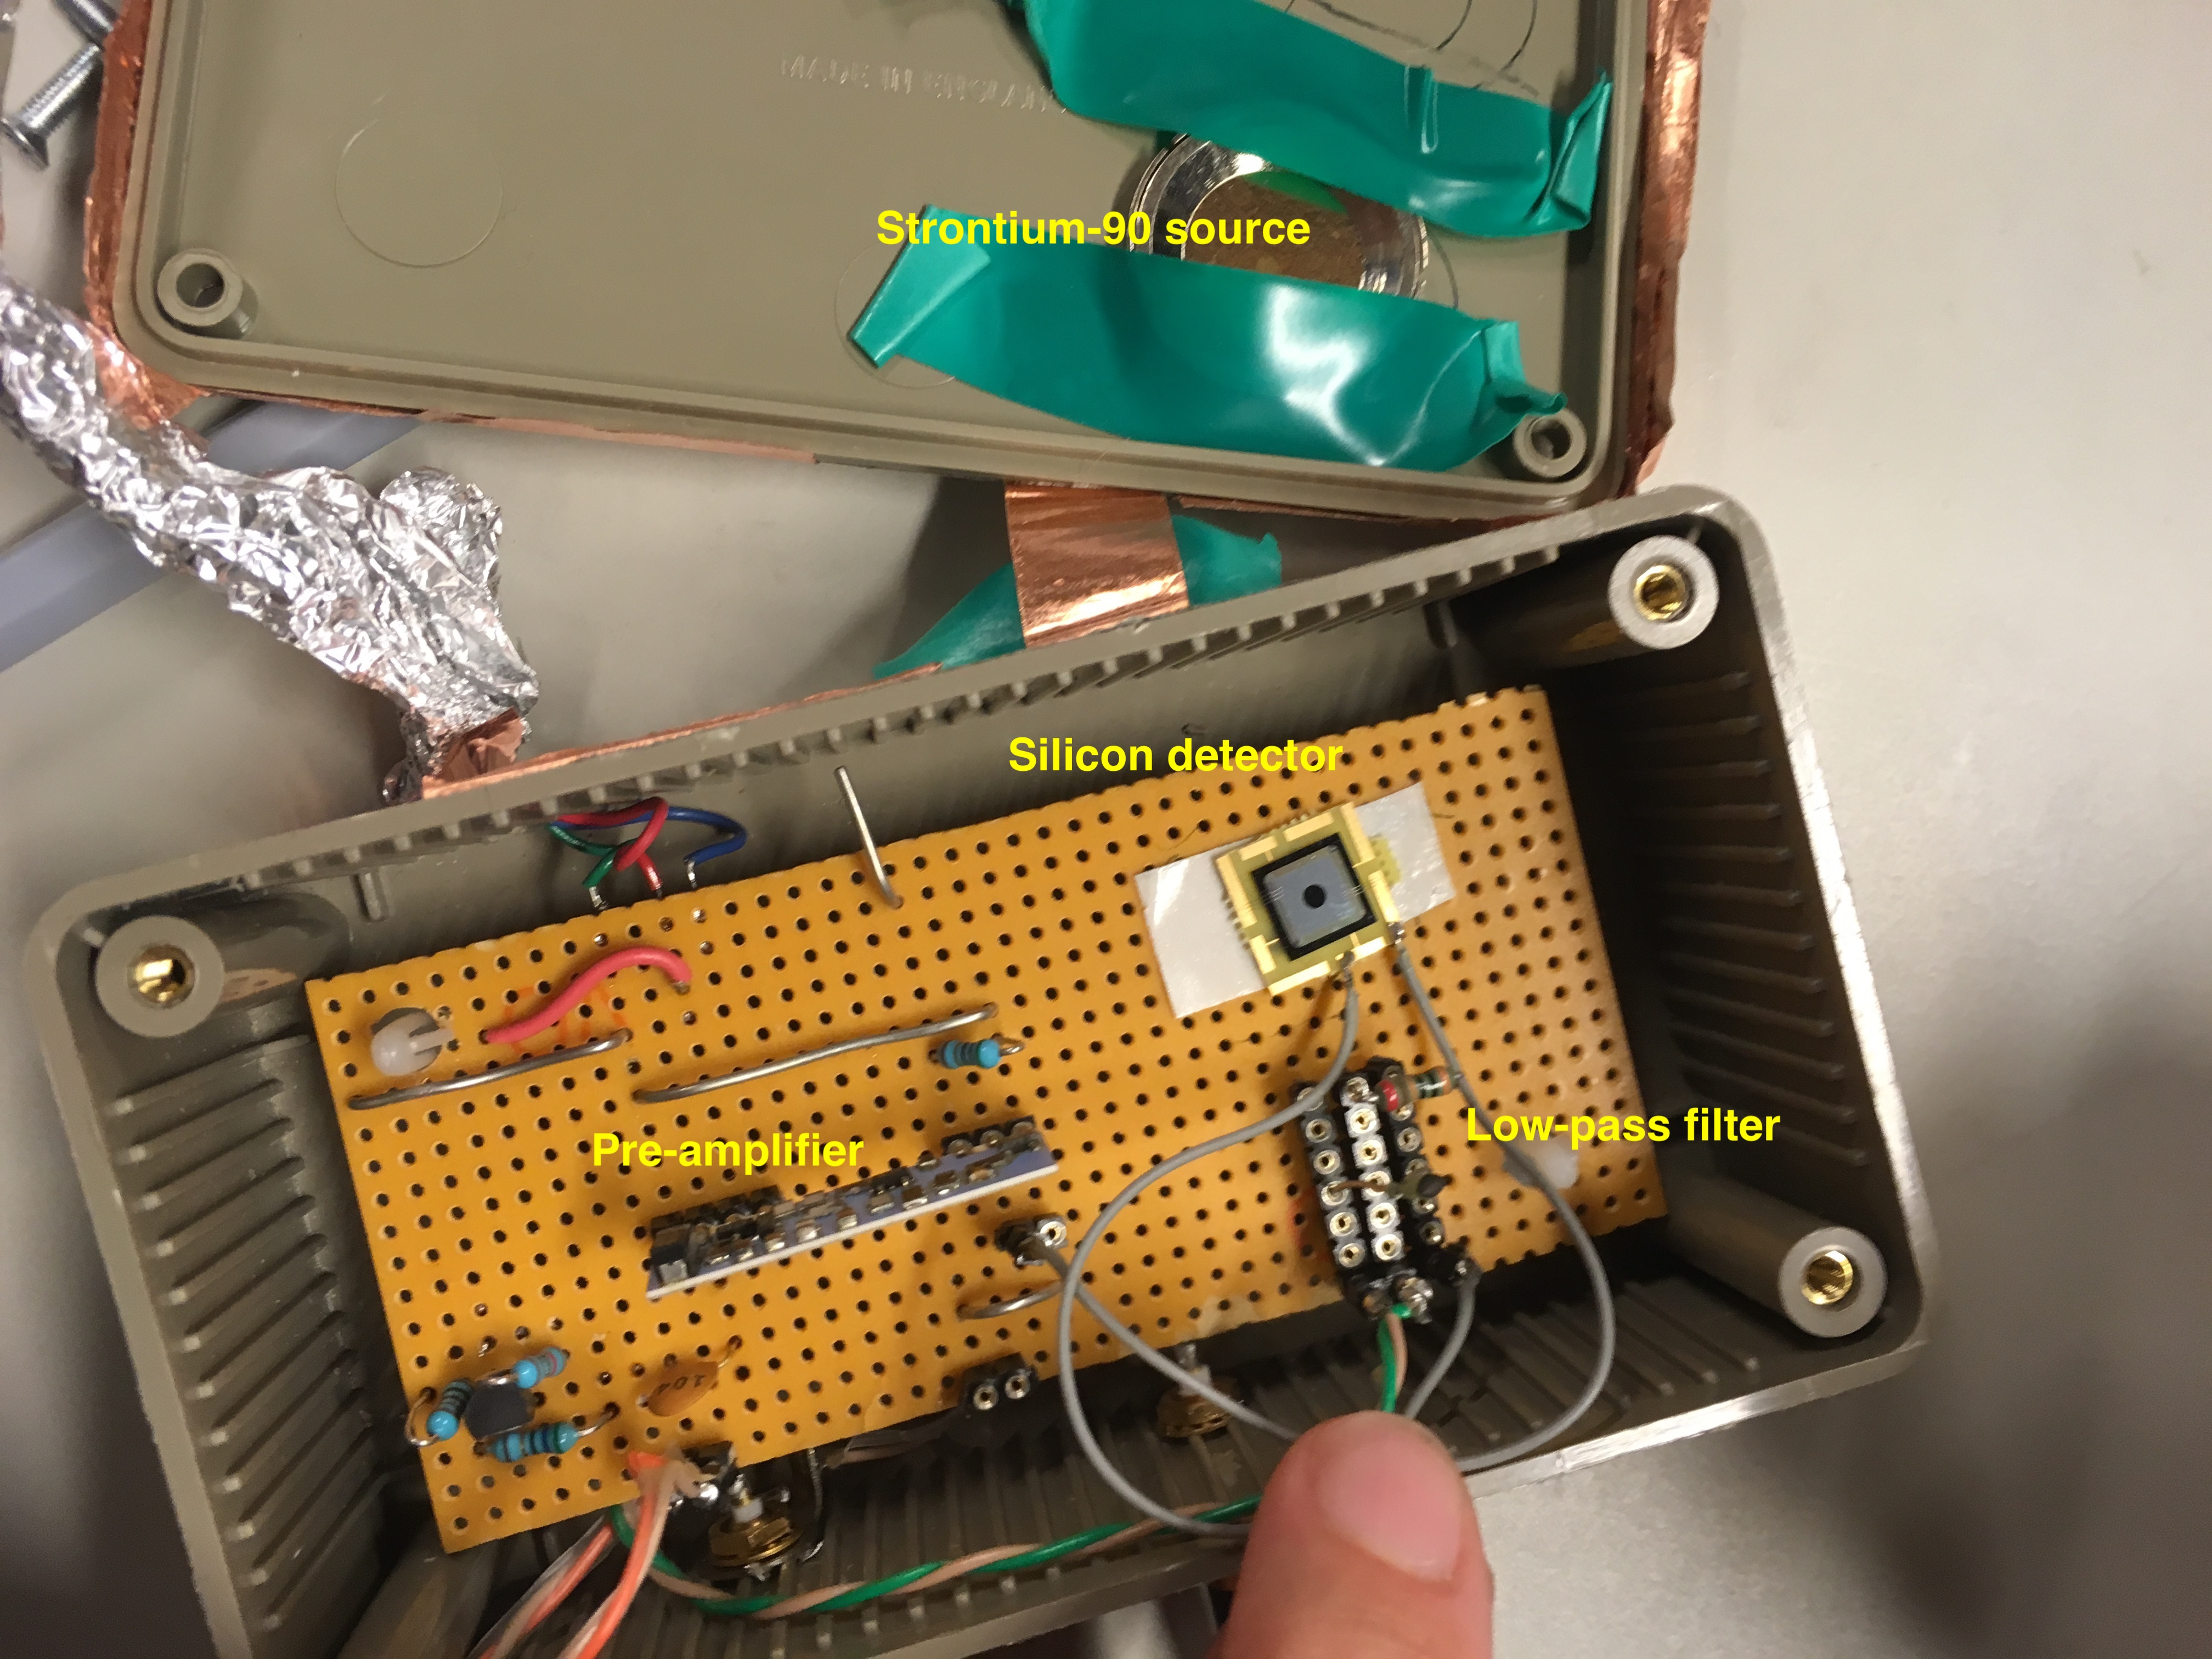
\includegraphics[width=\textwidth]{./graphics/experimentalSetup}
    \caption{}
    \label{fig:ExperimentalSetup}
  \end{subfigure}
  ~
  \begin{subfigure}[b]{0.45\textwidth}
    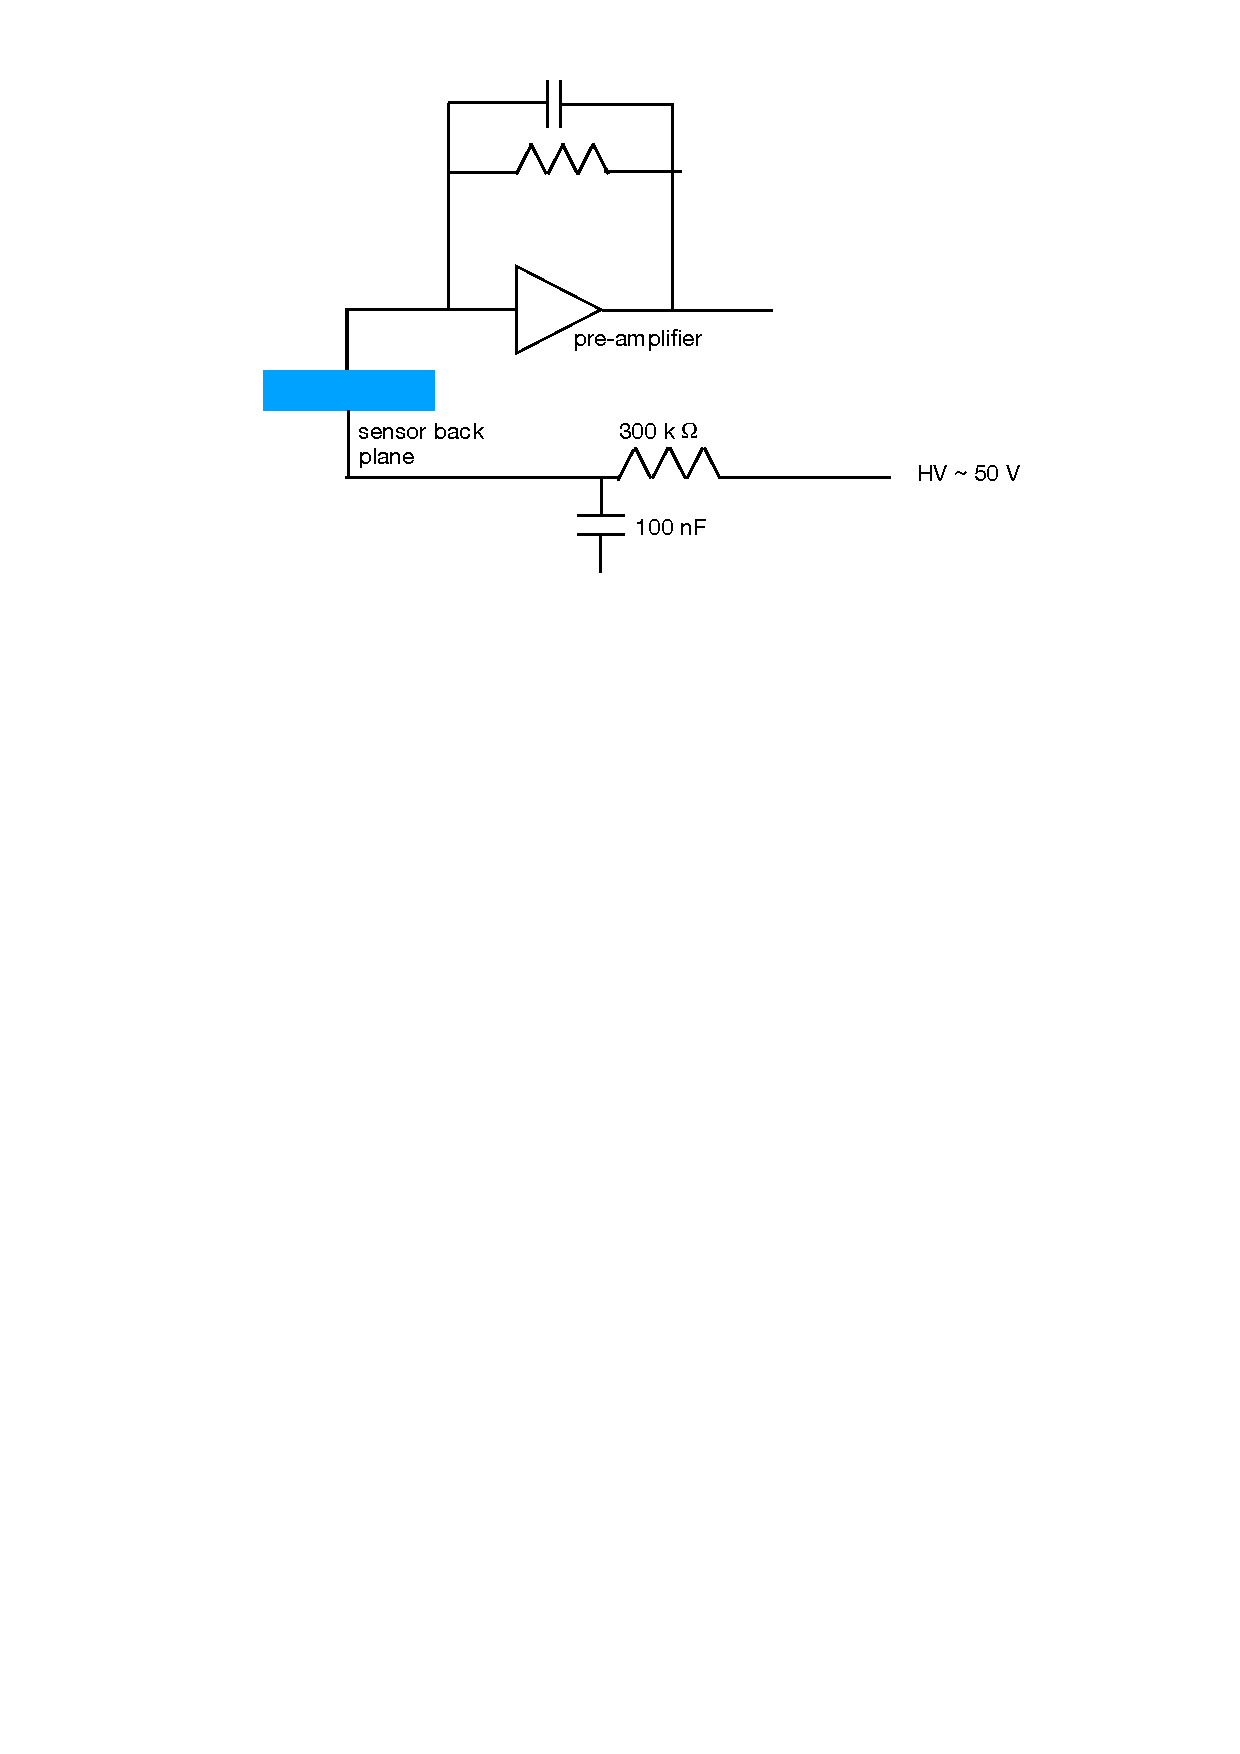
\includegraphics[width=\textwidth]{./graphics/SiliconDiodeCircuit}
    \caption{}
    \label{fig:SiliconDiodeCircuit}
  \end{subfigure}
  \caption{Silicon detector experimental setup. Left: photograph of the fully assembled circuit. Right: Schematics of the circuit with low-pass filter, pre-amplifier and silicon diode.}
\end{figure}


When one of the product decays of the radioactive source hit the diode, it induced a signal, which was observed on the oscilloscope. A few of these signals were saved and are visible in Figure \ref{fig:rise_time_measurement} and \ref{fig:rise_time_measurement_2}. Several measurements were extracted from these data. First of all the noise RMS was measured by taking the standard deviation of all the measured points before the pulse (until Time = $-0.5\mu$ s, which is a cut-off that is valid for all the datasets). The mean noise RMS for all the registered pulses and its uncertainty are $1.0 \pm 0.1$ mV.

\begin{figure}[h!]
  \centering
  \begin{subfigure}[t]{0.45\textwidth}
    \centering
    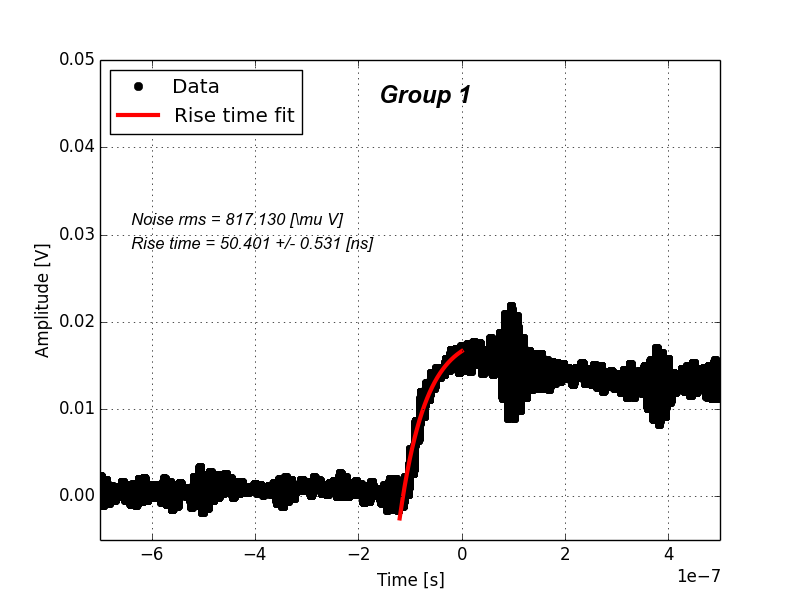
\includegraphics[width=1.1\textwidth]{./graphics/data_0.png}
  \end{subfigure}
  \hfill
  \begin{subfigure}[t]{0.45\textwidth}
    \centering
    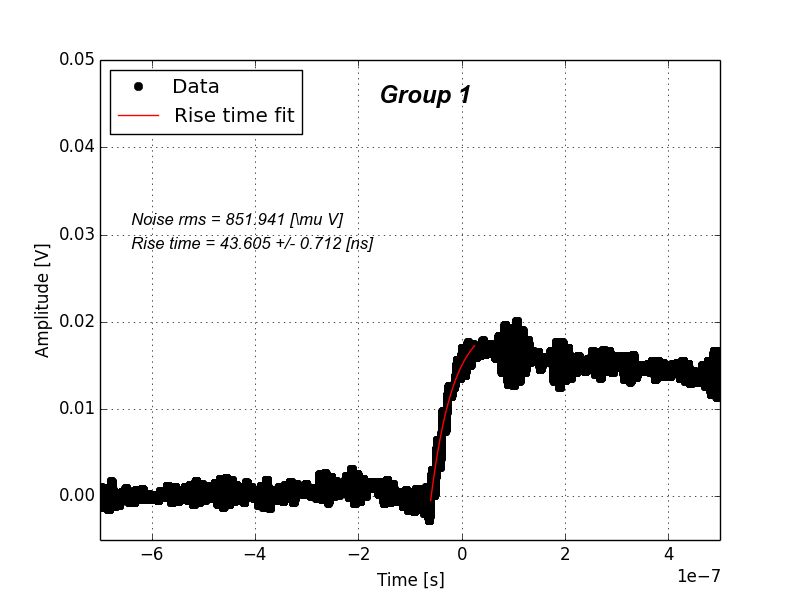
\includegraphics[width=1.1\textwidth]{./graphics/data_1.png}
  \end{subfigure}
  \hfill
  \begin{subfigure}[t]{0.45\textwidth}
    \centering
    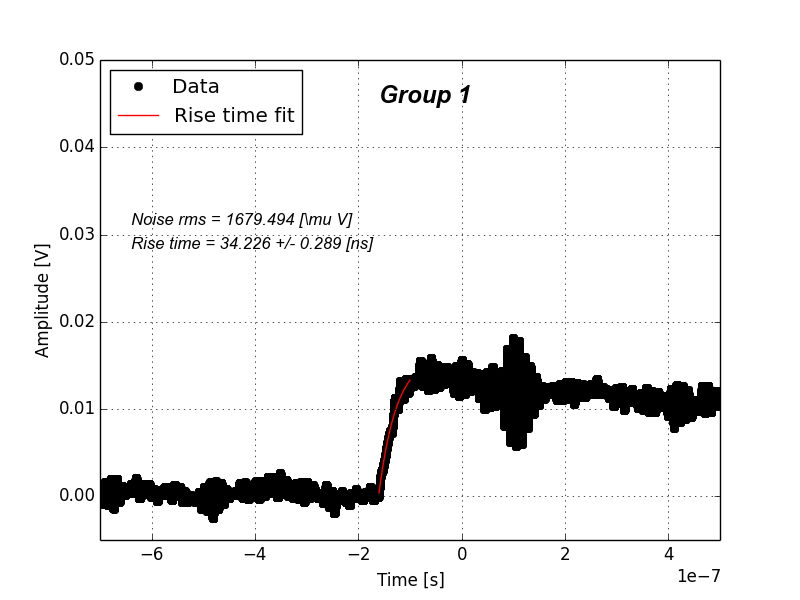
\includegraphics[width=1.1\textwidth]{./graphics/data_2.png}
  \end{subfigure}
  \hfill
  \begin{subfigure}[t]{0.45\textwidth}
    \centering
    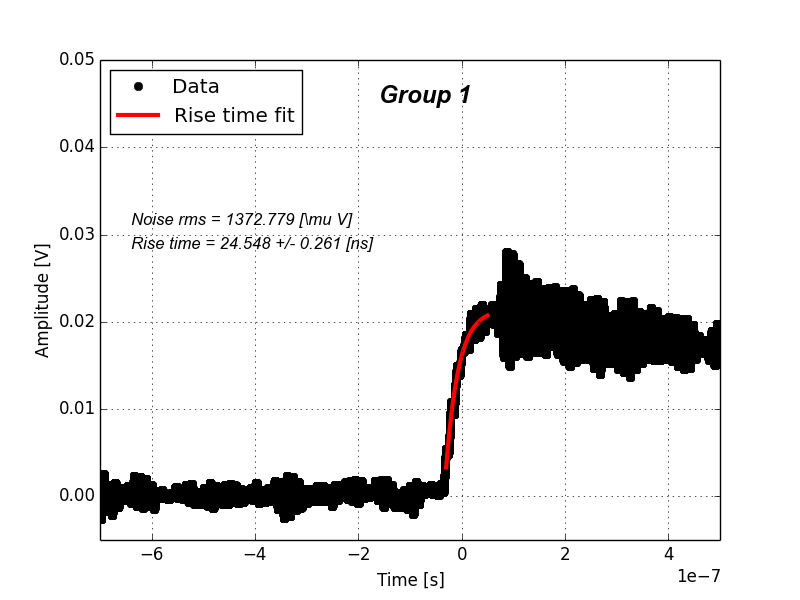
\includegraphics[width=1.1\textwidth]{./graphics/data_3.png}
  \end{subfigure}
  \hfill
  \begin{subfigure}[t]{0.45\textwidth}
    \centering
    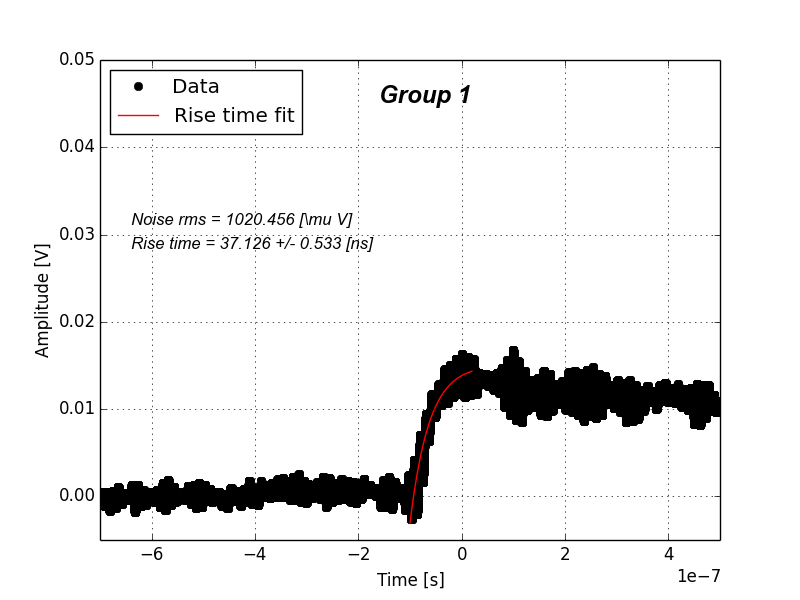
\includegraphics[width=1.1\textwidth]{./graphics/data_4.png}
  \end{subfigure}
  \hfill
  \begin{subfigure}[t]{0.45\textwidth}
    \centering
    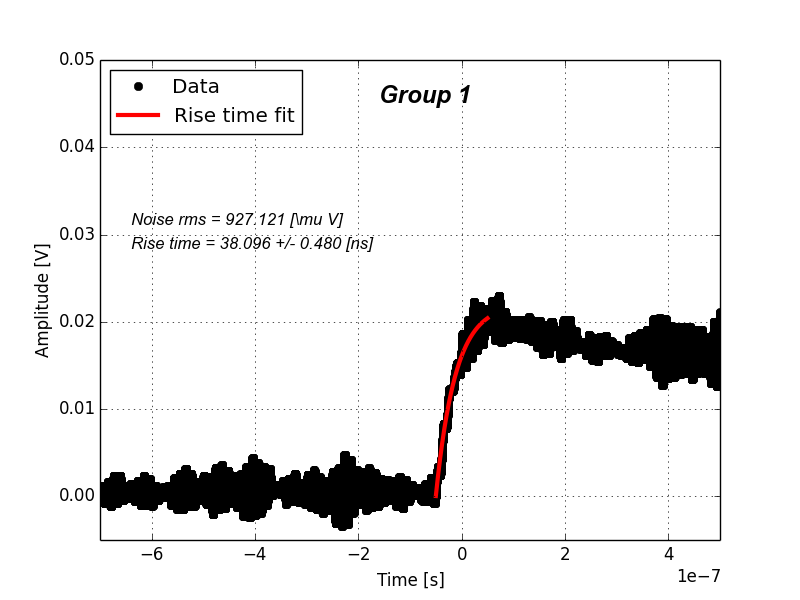
\includegraphics[width=1.1\textwidth]{./graphics/data_5.png}
  \end{subfigure}
\caption{Measurement of the rise time from the Strontium-90 decay. The red line is the fit (see Equation \ref{eq:rise_time}) to the data, while the highlighted green points are the data points used to measure the amplitude and its standard deviation and the blue points are the data used to evaluate the noise RMS}
\label{fig:rise_time_measurement}
\end{figure}
\begin{figure}[h!!]
  \centering
  \begin{subfigure}[t]{0.45\textwidth}
    \centering
    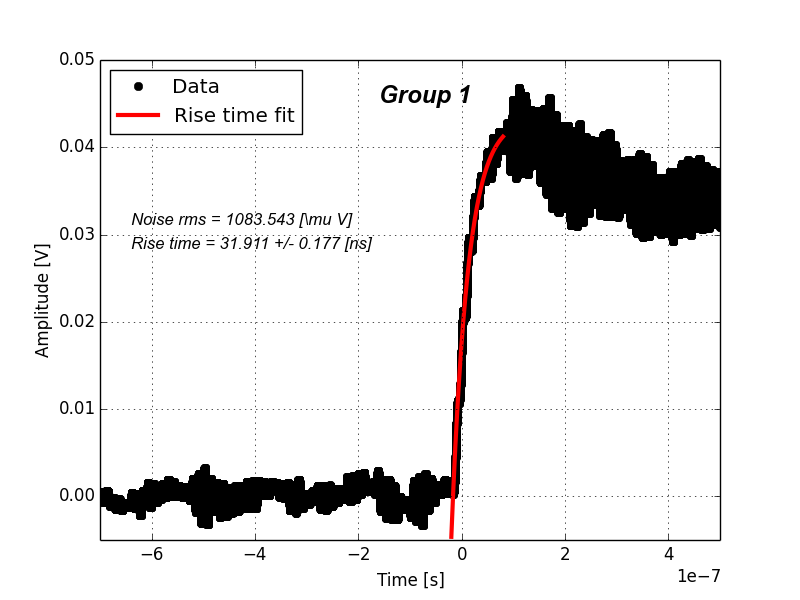
\includegraphics[width=1.1\textwidth]{./graphics/data_6.png}
  \end{subfigure}
  \hfill
  \begin{subfigure}[t]{0.45\textwidth}
    \centering
    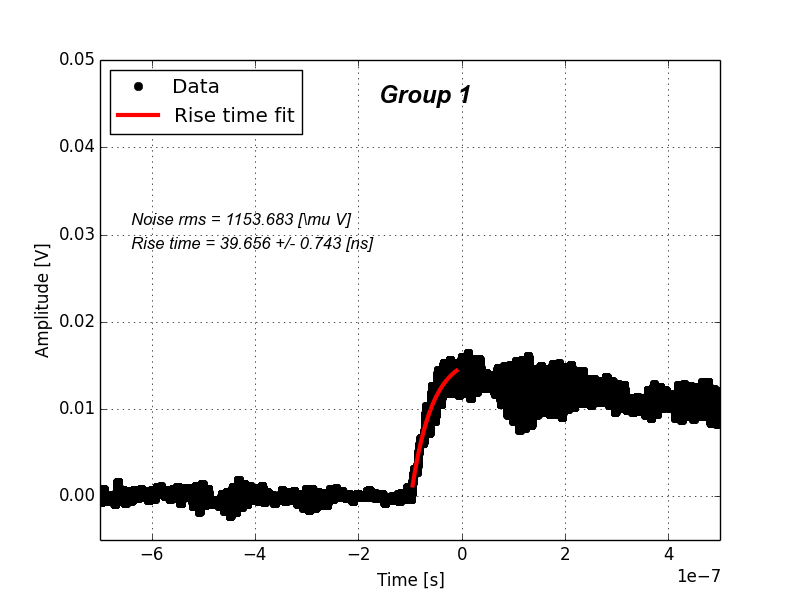
\includegraphics[width=1.1\textwidth]{./graphics/data_7.png}
  \end{subfigure}
  \hfill
  \begin{subfigure}[t]{0.45\textwidth}
    \centering
    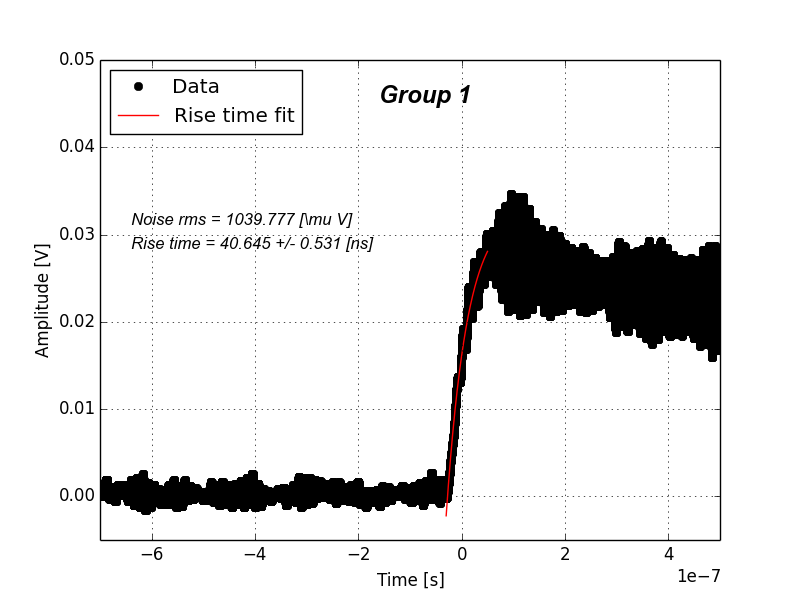
\includegraphics[width=1.1\textwidth]{./graphics/data_8.png}
  \end{subfigure}
  \hfill
  \begin{subfigure}[t]{0.45\textwidth}
    \centering
    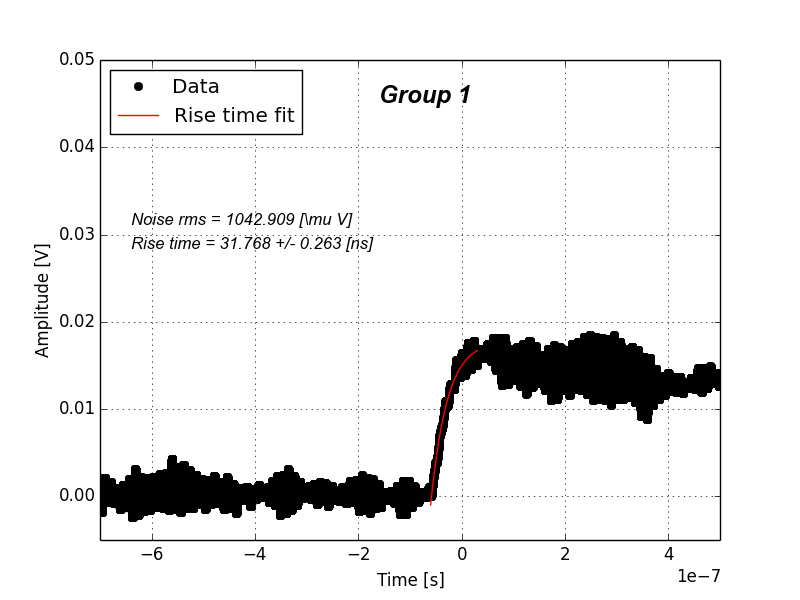
\includegraphics[width=1.1\textwidth]{./graphics/data_9.png}
  \end{subfigure}
  \hfill
  \begin{subfigure}[t]{0.45\textwidth}
    \centering
    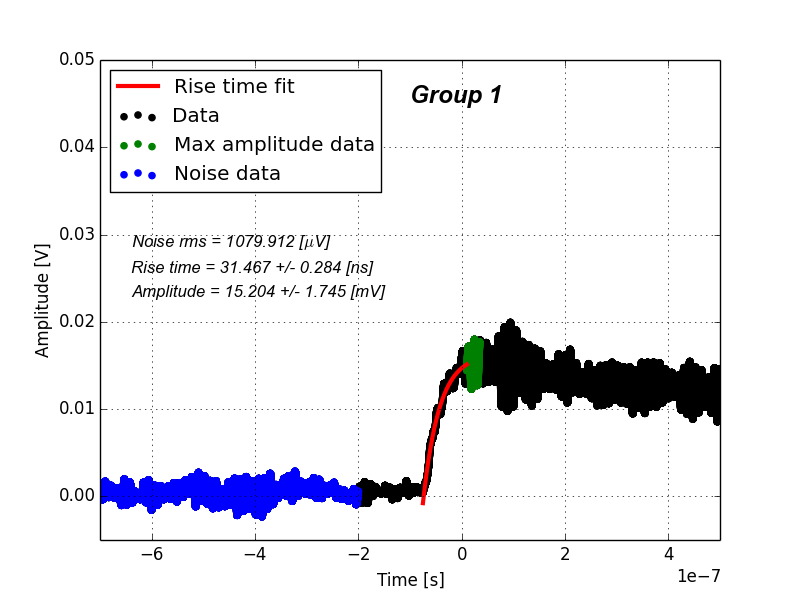
\includegraphics[width=1.1\textwidth]{./graphics/data_10.png}
  \end{subfigure}
  \hfill
  \begin{subfigure}[t]{0.45\textwidth}
    \centering
    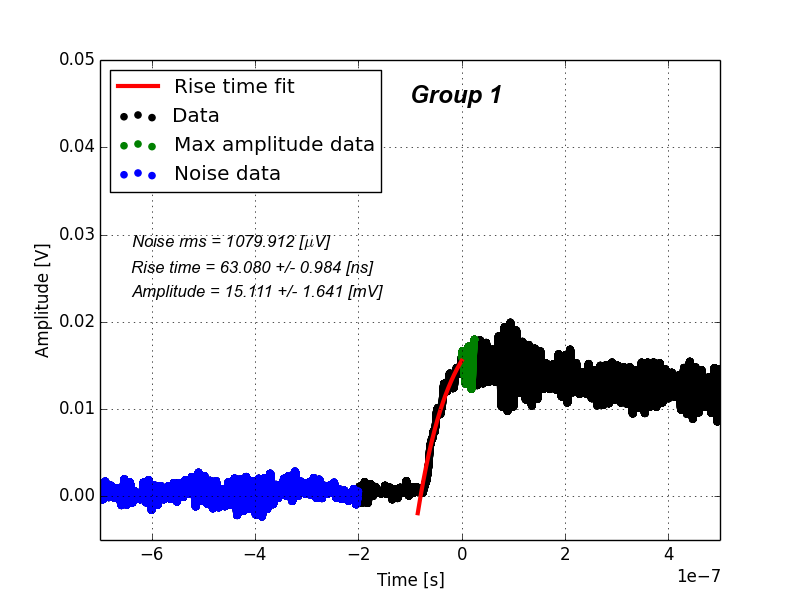
\includegraphics[width=1.1\textwidth]{./graphics/data_11.png}
  \end{subfigure}
\caption{Measurement of the rise time from the Strontium-90 decay. The red line is the fit (see Equation \ref{eq:rise_time}) to the data, while the highlighted green points are the data points used to measure the amplitude and its standard deviation and the blue points are the data used to evaluate the noise RMS}
\label{fig:rise_time_measurement_2}
\end{figure}

The rising pulse is fitted to find the rise time using the equation:
\begin{equation}
  V = V_{0} (1 - \exp^{-t/\tau}) + V_{noise}
  \label{eq:rise_time}
\end{equation}

where $V_{0}$ is the starting amplitude, $V_{noise}$ is the background amplitude and $\tau$ is the rising time. The rising time from the fit and the rising time from the calibration of the pre-amplifier are though not exactly the same rising time, as the first one is measured for the entire rising slope and the second one is measured only between $10\%$ and $90\%$ of the slope. In order to relate the two to each other, this relation exists:

\begin{equation}
t_{r} = \ln(9) \cdot \tau = 2.197 \cdot \tau
\end{equation}
where $t_{r}$ is the time interval between $10\%$ and $90\%$, while $\tau = RC$.

The mean rise time found with the fits is of $/tau = 38.9 \pm 9.7$ ns and if we multiply this by $2.197$ to get the time interval we get $t_{r} = 85.5 \pm 21.3$ ns. Using the mean rise time, we can extract the capacitance of the silicon detector system by extracting it from the parameters of the calibration curve on Figure \ref{fig:RiseTime_vs_Capacitance}. Given that the rise time calibration curve was fitted with a secon degree polynomial, we use the parameters there to isolate the capacitance term. The statistical uncertainty on the capacitance of the diode system is evaluated using a Monte Carlo technique with $100.000$ pseudoexperiments. Shortly, we draw $100.000$ different values for each parameter each from a Gaussian distribution, where the mean of the distribution is the value of the parameter and the standard deviation is the uncertainty of the parameter determined by the calibration fits. We solve the equation and find $100.000$ values of the capacitance. The statistical uncertainty is then estimated by taking the standard deviation of the gaussian fitted to the capacitance distribution, see Figure \ref{fig:stat_error_on_C}. The value of the diode system's capacitance is then C = $65 \pm 10$ pF.

\begin{figure}[h!]
  \centering
  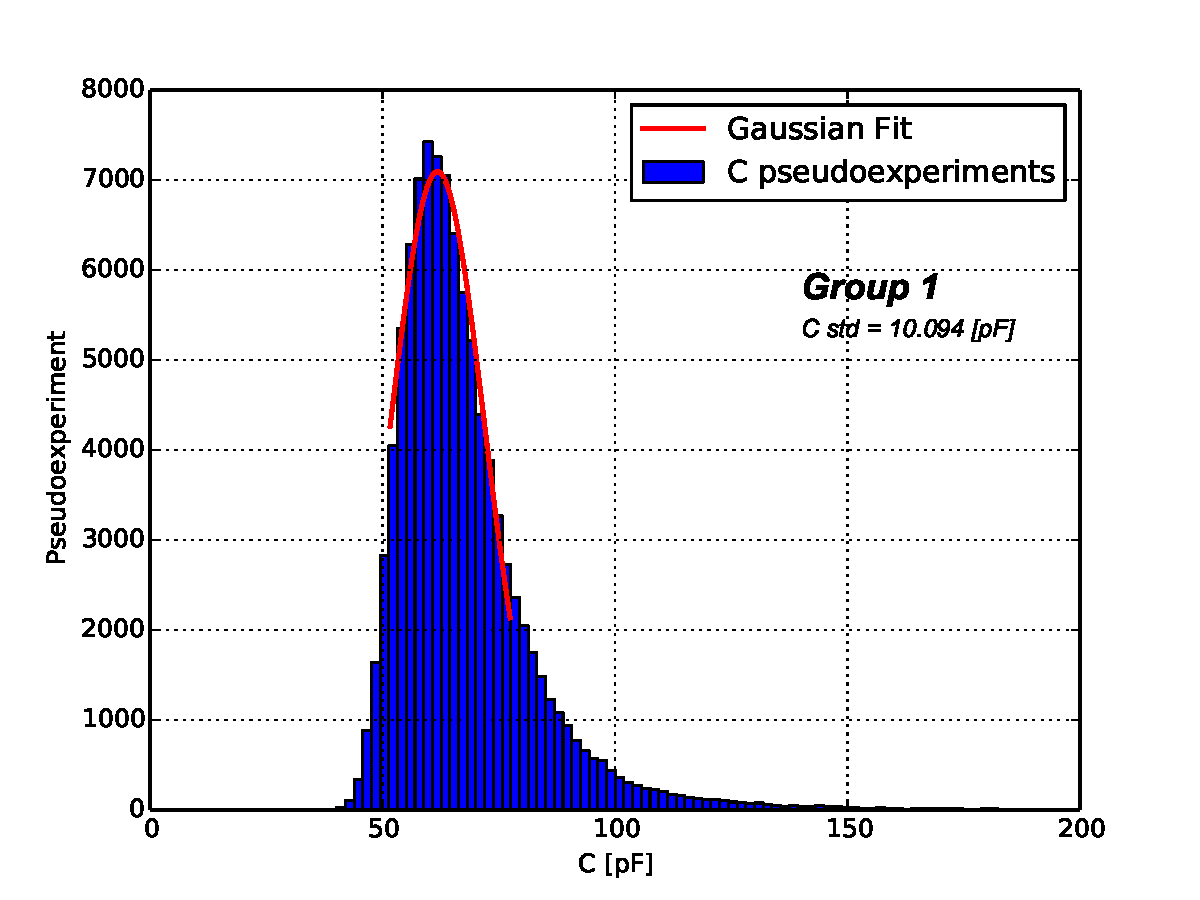
\includegraphics[width=0.8\textwidth]{./graphics/stat_error_on_C_pseudoexperiments}
  \caption{Statistical error on C from Monte Carlo pseudoexperiments}
  \label{fig:stat_error_on_C}
\end{figure}
%Given that the capacitance is found using a second degree coming from the calibration curve, the distribution of the value of the capacitance has a tail in one end. 

Using this extracted value of the capacitance, we can find the ENC of the silicon diode system by looking at the ENC calibration curve fit. The uncertainty is calculated using a simple error propagation, as we no longer have to solve a second order degree polynomial. The estimated value of the ENC is $42500 \pm 7700$ electrons.

Finally we extracted the pulse height from the measured Strontium-90 pulses and the values can be found in Figure \ref{fig:rise_time_measurement} and \ref{fig:rise_time_measurement_2}. The calibration pulses and the Strontium-90 pulses were measured with different oscilloscopes, which have different impedances. This results in a $40\%$ difference between the two pulses (with the calibration pulse being the highest). The amplitudes of the recorded Strontium-90 pulses are between $13$ mV and $41$ mV, which multiplied to $1.4$ gives an amplitude range between $18.2$ mV and $57.4$. Given the capacitance of the silicon diode system of $65$ pF, we can extrapolate from the amplitude vs capacitance dataset in Figure \ref{fig:Amplitude_vs_Capacitance} that we would expect an amplitude of between $30$ meV and $20$ meV, which fits the results observed in our experiment.


%################################################################################################
%
% Conclusion
%
%################################################################################################


\section{Conclusion}

In this experiment the preparation and characterisation of a silicon diode detector was observed, its depletion voltage and its capacitance have been measured. The pre-amplifier response was characterized and calibration curves were constructed by analysing the response of the pre-amplifier to a defined input pulse going through a set of dfferent capacitances. After connecting the diode to the pre-amplifier and radiating it with a radioactive source, we could measure, through the generated pulses by the detected charge, the sensor-preamplifier circuit's capacitance and ENC.



\end{document}
